\documentclass{beamer}

\usepackage{ctex}      %一个支持中文宏包,不用则中文无法正常显示
\usepackage{braket}    %狄拉克符号宏包,不需要用到时可删除
\usepackage{graphicx}  %通过宏包中的“\includegraphics”命令来插入图片
\graphicspath{{pics/}}  %图片所在路径设置,即图片放在一个名为“pics”的文件夹内,该文件夹与tex文件要在同一目录
\usepackage{subfigure}  %插入子图用
\setbeamertemplate{caption}[numbered]  %让插入的图片自动编号(beamer默认不编号)
\usefonttheme[onlymath]{serif}   %在公式中使用使用标准的Latex字体(有衬线的字体),区分小的L和大写的I
%beamer中默认使用Sans Serif字体,即没有衬线的字体
%\renewcommand{\thefootnote}{}    %取消脚注的编号,在后面花括号内添加其他符号也可改变脚注符号

\usetheme{Boadilla}      %幻灯片主题
\usecolortheme{default}  %主题的颜色
%可通过这个网站:https://hartwork.org/beamer-theme-matrix/  查看内置主题和颜色对应的效果

\AtBeginSection[]{
	\begin{frame}
		\tableofcontents[currentsection]
	\end{frame}
} %每到新的一节(Section)前就把目录显示一次

\title{Ballet算法的差分分析}                       %幻灯片标题
\author{张云帆\inst{1}, 肖康\inst{2}, 鲍国威\inst{3}, 刘世杰\inst{4}}        %作者
\institute{第1组 }  %单位,\and有换行的效果
\date{\today}                               %时间

\begin{document}     %开始正文
	\begin{frame}    %第一页PPT
		\titlepage   %将这一页设置为标题页
	\end{frame}
    
    \begin{frame}    %第二页PPT,目录页
    	\frametitle{目录}   %设置该页PPT的标题
    	\tableofcontents    %与\section{}一起使用制作目录,花括号里面的内容显示在目录页中
    \end{frame}
    
    \section{第一节}  %花括号的内容会显示在目录中
    \begin{frame}
    	\frametitle{本页幻灯片标题1}
    	\begin{figure}
    		\subfigure[aaa]{
    			
    		\begin{minipage}[t]{0.45\linewidth}   %0.45表示该部分内容占据长度为0.45倍的行宽
    		\centering                            %图片居中
    		
\includegraphics[scale=0.3]{1a}       %scale为图片缩放比例,根据实际图片大小调整
    		\label{fig1.sub1}
    		\end{minipage}
    	    }
            \subfigure[bbb]{  
            	\begin{minipage}[t]{0.45\linewidth}
            		\centering                     %图片居中
            		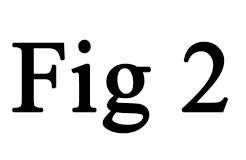
\includegraphics[scale=0.3]{1b}
            		\label{fig1.sub2}
            	\end{minipage}
            }
        \caption{图片命名1}
    	\end{figure}
    	正文……
    \end{frame}

    \begin{frame}
    	\frametitle{傅里叶变换}
    	算符傅里叶变换\footnote{\noindent\tiny{固体理论(第二版)-李正中-704011576X(ISBN)}}  %添加脚注
    	$$
    	\begin{aligned}
    	c_{nl}&=\frac{1}{\sqrt{N}}\sum_{k\in BZ}c_{nk}e^{i\vec{k}\cdot\vec{l}} \qquad c_{nk}=\frac{1}{\sqrt{N}}\sum_{l}c_{nl}e^{-i\vec{k}\cdot \vec{l}}  \\
    	c_{nl}^{\dagger}&=\frac{1}{\sqrt{N}}\sum_{k\in BZ}c_{nk}^{\dagger}e^{-i\vec{k}\cdot\vec{l}} \qquad c_{nk}^{\dagger}=\frac{1}{\sqrt{N}}\sum_{l}c_{nl}^{\dagger}e^{i\vec{k}\cdot \vec{l}} \\
    	~\\
    	\frac{1}{N}&\sum_{l}e^{\pm i(\vec{k}-\vec{k}')\cdot \vec{l}} = \delta_{kk'}; \qquad \frac{1}{N}\sum_{k\in BZ}e^{\pm i\vec{k}\cdot (\vec{l}-\vec{l}')}=\delta_{ll'}
    	\end{aligned}
    	$$
    \end{frame}

    \section{第二节}
	\begin{frame}
		\frametitle{本页幻灯片标题}
		正文
	\end{frame}
    
\end{document}